\documentclass[tikz,border=2mm]{standalone}
\usetikzlibrary{shapes.geometric, arrows.meta}

\tikzstyle{branching}=[circle, draw=blue, fill=blue!20]
\tikzstyle{red}=[circle, draw=red, fill=red!20]
\tikzstyle{orange}=[circle, draw=orange, fill=orange!20]

\begin{document}
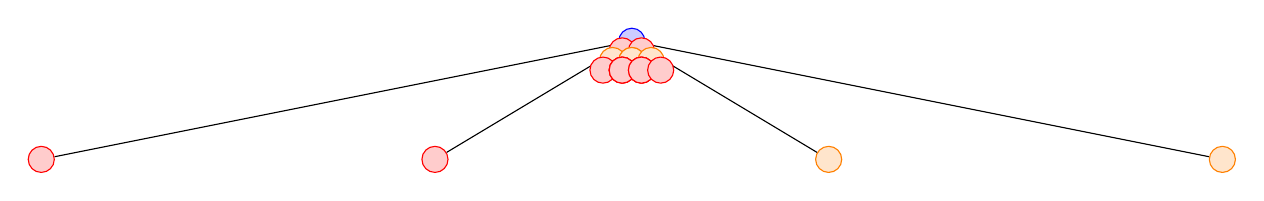
\begin{tikzpicture}[level/.style={sibling distance=5cm/#1}]
    % Root node (branching)
    \node[branching] (root) {}
        child {node[red] {}}
        child {node[red] {}}
        child {node[orange] {}}
        child {node[orange] {}};

    % Level 2 nodes
    \node[red] (child1) at (root.south west) {};
    \node[red] (child2) at (root.south east) {};
    \node[orange] (child3) at (child1.south west) {};
    \node[orange] (child4) at (child1.south east) {};
    \node[orange] (child5) at (child2.south west) {};
    \node[orange] (child6) at (child2.south east) {};

    % Level 3 nodes
    \node[red] (grandchild1) at (child3.south west) {};
    \node[red] (grandchild2) at (child3.south east) {};
    \node[red] (grandchild3) at (child4.south west) {};
    \node[red] (grandchild4) at (child4.south east) {};
    \node[red] (grandchild5) at (child5.south west) {};
    \node[red] (grandchild6) at (child5.south east) {};
    \node[red] (grandchild7) at (child6.south west) {};
    \node[red] (grandchild8) at (child6.south east) {};
\end{tikzpicture}
\end{document}